\documentclass[1p]{elsarticle_modified}
%\bibliographystyle{elsarticle-num}

%\usepackage[colorlinks]{hyperref}
%\usepackage{abbrmath_seonhwa} %\Abb, \Ascr, \Acal ,\Abf, \Afrak
\usepackage{amsfonts}
\usepackage{amssymb}
\usepackage{amsmath}
\usepackage{amsthm}
\usepackage{scalefnt}
\usepackage{amsbsy}
\usepackage{kotex}
\usepackage{caption}
\usepackage{subfig}
\usepackage{color}
\usepackage{graphicx}
\usepackage{xcolor} %% white, black, red, green, blue, cyan, magenta, yellow
\usepackage{float}
\usepackage{setspace}
\usepackage{hyperref}

\usepackage{tikz}
\usetikzlibrary{arrows}

\usepackage{multirow}
\usepackage{array} % fixed length table
\usepackage{hhline}

%%%%%%%%%%%%%%%%%%%%%
\makeatletter
\renewcommand*\env@matrix[1][\arraystretch]{%
	\edef\arraystretch{#1}%
	\hskip -\arraycolsep
	\let\@ifnextchar\new@ifnextchar
	\array{*\c@MaxMatrixCols c}}
\makeatother %https://tex.stackexchange.com/questions/14071/how-can-i-increase-the-line-spacing-in-a-matrix
%%%%%%%%%%%%%%%

\usepackage[normalem]{ulem}

\newcommand{\msout}[1]{\ifmmode\text{\sout{\ensuremath{#1}}}\else\sout{#1}\fi}
%SOURCE: \msout is \stkout macro in https://tex.stackexchange.com/questions/20609/strikeout-in-math-mode

\newcommand{\cancel}[1]{
	\ifmmode
	{\color{red}\msout{#1}}
	\else
	{\color{red}\sout{#1}}
	\fi
}

\newcommand{\add}[1]{
	{\color{blue}\uwave{#1}}
}

\newcommand{\replace}[2]{
	\ifmmode
	{\color{red}\msout{#1}}{\color{blue}\uwave{#2}}
	\else
	{\color{red}\sout{#1}}{\color{blue}\uwave{#2}}
	\fi
}

\newcommand{\Sol}{\mathcal{S}} %segment
\newcommand{\D}{D} %diagram
\newcommand{\A}{\mathcal{A}} %arc


%%%%%%%%%%%%%%%%%%%%%%%%%%%%%5 test

\def\sl{\operatorname{\textup{SL}}(2,\Cbb)}
\def\psl{\operatorname{\textup{PSL}}(2,\Cbb)}
\def\quan{\mkern 1mu \triangleright \mkern 1mu}

\theoremstyle{definition}
\newtheorem{thm}{Theorem}[section]
\newtheorem{prop}[thm]{Proposition}
\newtheorem{lem}[thm]{Lemma}
\newtheorem{ques}[thm]{Question}
\newtheorem{cor}[thm]{Corollary}
\newtheorem{defn}[thm]{Definition}
\newtheorem{exam}[thm]{Example}
\newtheorem{rmk}[thm]{Remark}
\newtheorem{alg}[thm]{Algorithm}

\newcommand{\I}{\sqrt{-1}}
\begin{document}

%\begin{frontmatter}
%
%\title{Boundary parabolic representations of knots up to 8 crossings}
%
%%% Group authors per affiliation:
%\author{Yunhi Cho} 
%\address{Department of Mathematics, University of Seoul, Seoul, Korea}
%\ead{yhcho@uos.ac.kr}
%
%
%\author{Seonhwa Kim} %\fnref{s_kim}}
%\address{Center for Geometry and Physics, Institute for Basic Science, Pohang, 37673, Korea}
%\ead{ryeona17@ibs.re.kr}
%
%\author{Hyuk Kim}
%\address{Department of Mathematical Sciences, Seoul National University, Seoul 08826, Korea}
%\ead{hyukkim@snu.ac.kr}
%
%\author{Seokbeom Yoon}
%\address{Department of Mathematical Sciences, Seoul National University, Seoul, 08826,  Korea}
%\ead{sbyoon15@snu.ac.kr}
%
%\begin{abstract}
%We find all boundary parabolic representation of knots up to 8 crossings.
%
%\end{abstract}
%\begin{keyword}
%    \MSC[2010] 57M25 
%\end{keyword}
%
%\end{frontmatter}

%\linenumbers
%\tableofcontents
%
\newcommand\colored[1]{\textcolor{white}{\rule[-0.35ex]{0.8em}{1.4ex}}\kern-0.8em\color{red} #1}%
%\newcommand\colored[1]{\textcolor{white}{ #1}\kern-2.17ex	\textcolor{white}{ #1}\kern-1.81ex	\textcolor{white}{ #1}\kern-2.15ex\color{red}#1	}

{\Large $\underline{12a_{0535}~(K12a_{0535})}$}

\setlength{\tabcolsep}{10pt}
\renewcommand{\arraystretch}{1.6}
\vspace{1cm}\begin{tabular}{m{100pt}>{\centering\arraybackslash}m{274pt}}
\multirow{5}{120pt}{
	\centering
	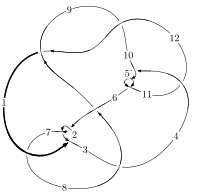
\includegraphics[width=112pt]{../../../GIT/diagram.site/Diagrams/png/1336_12a_0535.png}\\
\ \ \ A knot diagram\footnotemark}&
\allowdisplaybreaks
\textbf{Linearized knot diagam} \\
\cline{2-2}
 &
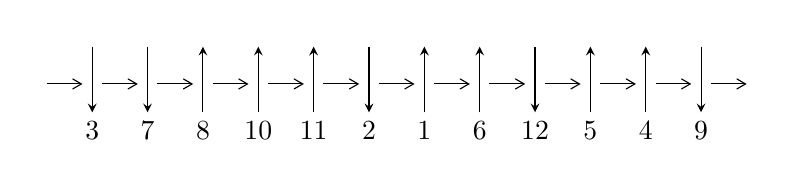
\begin{tikzpicture}[x=20pt, y=17pt]
	% nodes
	\node (C0) at (0, 0) {};
	\node (C1) at (1, 0) {};
	\node (C1U) at (1, +1) {};
	\node (C1D) at (1, -1) {3};

	\node (C2) at (2, 0) {};
	\node (C2U) at (2, +1) {};
	\node (C2D) at (2, -1) {7};

	\node (C3) at (3, 0) {};
	\node (C3U) at (3, +1) {};
	\node (C3D) at (3, -1) {8};

	\node (C4) at (4, 0) {};
	\node (C4U) at (4, +1) {};
	\node (C4D) at (4, -1) {10};

	\node (C5) at (5, 0) {};
	\node (C5U) at (5, +1) {};
	\node (C5D) at (5, -1) {11};

	\node (C6) at (6, 0) {};
	\node (C6U) at (6, +1) {};
	\node (C6D) at (6, -1) {2};

	\node (C7) at (7, 0) {};
	\node (C7U) at (7, +1) {};
	\node (C7D) at (7, -1) {1};

	\node (C8) at (8, 0) {};
	\node (C8U) at (8, +1) {};
	\node (C8D) at (8, -1) {6};

	\node (C9) at (9, 0) {};
	\node (C9U) at (9, +1) {};
	\node (C9D) at (9, -1) {12};

	\node (C10) at (10, 0) {};
	\node (C10U) at (10, +1) {};
	\node (C10D) at (10, -1) {5};

	\node (C11) at (11, 0) {};
	\node (C11U) at (11, +1) {};
	\node (C11D) at (11, -1) {4};

	\node (C12) at (12, 0) {};
	\node (C12U) at (12, +1) {};
	\node (C12D) at (12, -1) {9};
	\node (C13) at (13, 0) {};

	% arrows
	\draw[->,>={angle 60}]
	(C0) edge (C1) (C1) edge (C2) (C2) edge (C3) (C3) edge (C4) (C4) edge (C5) (C5) edge (C6) (C6) edge (C7) (C7) edge (C8) (C8) edge (C9) (C9) edge (C10) (C10) edge (C11) (C11) edge (C12) (C12) edge (C13) ;	\draw[->,>=stealth]
	(C1U) edge (C1D) (C2U) edge (C2D) (C3D) edge (C3U) (C4D) edge (C4U) (C5D) edge (C5U) (C6U) edge (C6D) (C7D) edge (C7U) (C8D) edge (C8U) (C9U) edge (C9D) (C10D) edge (C10U) (C11D) edge (C11U) (C12U) edge (C12D) ;
	\end{tikzpicture} \\
\hhline{~~} \\& 
\textbf{Solving Sequence} \\ \cline{2-2} 
 &
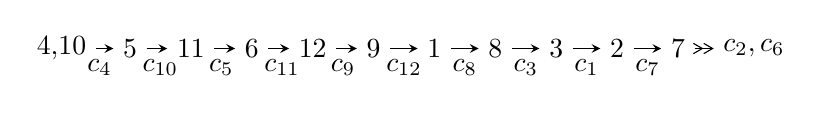
\begin{tikzpicture}[x=22pt, y=7pt]
	% node
	\node (A0) at (-1/8, 0) {4,10};
	\node (A1) at (1, 0) {5};
	\node (A2) at (2, 0) {11};
	\node (A3) at (3, 0) {6};
	\node (A4) at (4, 0) {12};
	\node (A5) at (5, 0) {9};
	\node (A6) at (6, 0) {1};
	\node (A7) at (7, 0) {8};
	\node (A8) at (8, 0) {3};
	\node (A9) at (9, 0) {2};
	\node (A10) at (10, 0) {7};
	\node (C1) at (1/2, -1) {$c_{4}$};
	\node (C2) at (3/2, -1) {$c_{10}$};
	\node (C3) at (5/2, -1) {$c_{5}$};
	\node (C4) at (7/2, -1) {$c_{11}$};
	\node (C5) at (9/2, -1) {$c_{9}$};
	\node (C6) at (11/2, -1) {$c_{12}$};
	\node (C7) at (13/2, -1) {$c_{8}$};
	\node (C8) at (15/2, -1) {$c_{3}$};
	\node (C9) at (17/2, -1) {$c_{1}$};
	\node (C10) at (19/2, -1) {$c_{7}$};
	\node (A11) at (45/4, 0) {$c_{2},c_{6}$};

	% edge
	\draw[->,>=stealth]	
	(A0) edge (A1) (A1) edge (A2) (A2) edge (A3) (A3) edge (A4) (A4) edge (A5) (A5) edge (A6) (A6) edge (A7) (A7) edge (A8) (A8) edge (A9) (A9) edge (A10) ;
	\draw[->>,>={angle 60}]	
	(A10) edge (A11);
\end{tikzpicture} \\ 

\end{tabular} \\

\footnotetext{
The image of knot diagram is generated by the software ``\textbf{Draw programme}" developed by Andrew Bartholomew(\url{http://www.layer8.co.uk/maths/draw/index.htm\#Running-draw}), where we modified some parts for our purpose(\url{https://github.com/CATsTAILs/LinksPainter}).
}\phantom \\ \newline 
\centering \textbf{Ideals for irreducible components\footnotemark of $X_{\text{par}}$} 
 
\begin{align*}
I^u_{1}&=\langle 
u^{87}- u^{86}+\cdots+2 u^3+1\rangle \\
\\
\end{align*}
\raggedright * 1 irreducible components of $\dim_{\mathbb{C}}=0$, with total 87 representations.\\
\footnotetext{All coefficients of polynomials are rational numbers. But the coefficients are sometimes approximated in decimal forms when there is not enough margin.}
\newpage
\renewcommand{\arraystretch}{1}
\centering \section*{I. $I^u_{1}= \langle u^{87}- u^{86}+\cdots+2 u^3+1 \rangle$}
\flushleft \textbf{(i) Arc colorings}\\
\begin{tabular}{m{7pt} m{180pt} m{7pt} m{180pt} }
\flushright $a_{4}=$&$\begin{pmatrix}1\\0\end{pmatrix}$ \\
\flushright $a_{10}=$&$\begin{pmatrix}0\\u\end{pmatrix}$ \\
\flushright $a_{5}=$&$\begin{pmatrix}1\\- u^2\end{pmatrix}$ \\
\flushright $a_{11}=$&$\begin{pmatrix}u\\- u^3+u\end{pmatrix}$ \\
\flushright $a_{6}=$&$\begin{pmatrix}- u^2+1\\u^4-2 u^2\end{pmatrix}$ \\
\flushright $a_{12}=$&$\begin{pmatrix}- u^3+2 u\\- u^3+u\end{pmatrix}$ \\
\flushright $a_{9}=$&$\begin{pmatrix}u^7-4 u^5+4 u^3\\u^7-3 u^5+2 u^3+u\end{pmatrix}$ \\
\flushright $a_{1}=$&$\begin{pmatrix}- u^{11}+6 u^9-12 u^7+8 u^5- u^3+2 u\\- u^{11}+5 u^9-8 u^7+3 u^5+u^3+u\end{pmatrix}$ \\
\flushright $a_{8}=$&$\begin{pmatrix}- u^{13}+6 u^{11}-13 u^9+12 u^7-6 u^5+4 u^3- u\\u^{15}-7 u^{13}+18 u^{11}-19 u^9+6 u^7-2 u^5+4 u^3+u\end{pmatrix}$ \\
\flushright $a_{3}=$&$\begin{pmatrix}- u^{28}+13 u^{26}+\cdots- u^2+1\\u^{30}-14 u^{28}+\cdots+8 u^4+u^2\end{pmatrix}$ \\
\flushright $a_{2}=$&$\begin{pmatrix}u^{69}-32 u^{67}+\cdots+2 u^3+u\\- u^{71}+33 u^{69}+\cdots-3 u^5+u\end{pmatrix}$ \\
\flushright $a_{7}=$&$\begin{pmatrix}- u^{37}+18 u^{35}+\cdots-2 u^3- u\\- u^{37}+17 u^{35}+\cdots+u^3+u\end{pmatrix}$\\&\end{tabular}
\flushleft \textbf{(ii) Obstruction class $= -1$}\\~\\
\flushleft \textbf{(iii) Cusp Shapes $= -4 u^{85}+160 u^{83}+\cdots+4 u^2+2$}\\~\\
\newpage\renewcommand{\arraystretch}{1}
\flushleft \textbf{(iv) u-Polynomials at the component}\newline \\
\begin{tabular}{m{50pt}|m{274pt}}
Crossings & \hspace{64pt}u-Polynomials at each crossing \\
\hline $$\begin{aligned}c_{1}\end{aligned}$$&$\begin{aligned}
&u^{87}+41 u^{86}+\cdots+2 u^2+1
\end{aligned}$\\
\hline $$\begin{aligned}c_{2},c_{6}\end{aligned}$$&$\begin{aligned}
&u^{87}- u^{86}+\cdots+2 u-1
\end{aligned}$\\
\hline $$\begin{aligned}c_{3}\end{aligned}$$&$\begin{aligned}
&u^{87}+u^{86}+\cdots+200 u-676
\end{aligned}$\\
\hline $$\begin{aligned}c_{4},c_{5},c_{10}\end{aligned}$$&$\begin{aligned}
&u^{87}+u^{86}+\cdots+2 u^3-1
\end{aligned}$\\
\hline $$\begin{aligned}c_{7}\end{aligned}$$&$\begin{aligned}
&u^{87}-3 u^{86}+\cdots+1868 u-369
\end{aligned}$\\
\hline $$\begin{aligned}c_{8}\end{aligned}$$&$\begin{aligned}
&u^{87}+11 u^{86}+\cdots-4 u+1
\end{aligned}$\\
\hline $$\begin{aligned}c_{9},c_{12}\end{aligned}$$&$\begin{aligned}
&u^{87}-13 u^{86}+\cdots+672 u-23
\end{aligned}$\\
\hline $$\begin{aligned}c_{11}\end{aligned}$$&$\begin{aligned}
&u^{87}-3 u^{86}+\cdots-760 u+1491
\end{aligned}$\\
\hline
\end{tabular}\\~\\
\newpage\renewcommand{\arraystretch}{1}
\flushleft \textbf{(v) Riley Polynomials at the component}\newline \\
\begin{tabular}{m{50pt}|m{274pt}}
Crossings & \hspace{64pt}Riley Polynomials at each crossing \\
\hline $$\begin{aligned}c_{1}\end{aligned}$$&$\begin{aligned}
&y^{87}+11 y^{86}+\cdots-4 y-1
\end{aligned}$\\
\hline $$\begin{aligned}c_{2},c_{6}\end{aligned}$$&$\begin{aligned}
&y^{87}-41 y^{86}+\cdots-2 y^2-1
\end{aligned}$\\
\hline $$\begin{aligned}c_{3}\end{aligned}$$&$\begin{aligned}
&y^{87}-25 y^{86}+\cdots+2553368 y-456976
\end{aligned}$\\
\hline $$\begin{aligned}c_{4},c_{5},c_{10}\end{aligned}$$&$\begin{aligned}
&y^{87}-81 y^{86}+\cdots+6 y^2-1
\end{aligned}$\\
\hline $$\begin{aligned}c_{7}\end{aligned}$$&$\begin{aligned}
&y^{87}+19 y^{86}+\cdots-3993896 y-136161
\end{aligned}$\\
\hline $$\begin{aligned}c_{8}\end{aligned}$$&$\begin{aligned}
&y^{87}- y^{86}+\cdots+276 y-1
\end{aligned}$\\
\hline $$\begin{aligned}c_{9},c_{12}\end{aligned}$$&$\begin{aligned}
&y^{87}+71 y^{86}+\cdots-2068 y-529
\end{aligned}$\\
\hline $$\begin{aligned}c_{11}\end{aligned}$$&$\begin{aligned}
&y^{87}-29 y^{86}+\cdots+72372232 y-2223081
\end{aligned}$\\
\hline
\end{tabular}\\~\\
\newpage\flushleft \textbf{(vi) Complex Volumes and Cusp Shapes}
$$\begin{array}{c|c|c}  
\text{Solutions to }I^u_{1}& \I (\text{vol} + \sqrt{-1}CS) & \text{Cusp shape}\\
 \hline 
\begin{aligned}
u &= \phantom{-}1.156780 + 0.129439 I\end{aligned}
 & -0.70238 - 4.44670 I & \phantom{-0.000000 } 0 \\ \hline\begin{aligned}
u &= \phantom{-}1.156780 - 0.129439 I\end{aligned}
 & -0.70238 + 4.44670 I & \phantom{-0.000000 } 0 \\ \hline\begin{aligned}
u &= -1.190410 + 0.114228 I\end{aligned}
 & \phantom{-}1.68051 - 0.08481 I & \phantom{-0.000000 } 0 \\ \hline\begin{aligned}
u &= -1.190410 - 0.114228 I\end{aligned}
 & \phantom{-}1.68051 + 0.08481 I & \phantom{-0.000000 } 0 \\ \hline\begin{aligned}
u &= \phantom{-}1.197740 + 0.161716 I\end{aligned}
 & -2.06048 + 3.05466 I & \phantom{-0.000000 } 0 \\ \hline\begin{aligned}
u &= \phantom{-}1.197740 - 0.161716 I\end{aligned}
 & -2.06048 - 3.05466 I & \phantom{-0.000000 } 0 \\ \hline\begin{aligned}
u &= -0.394345 + 0.684266 I\end{aligned}
 & \phantom{-}1.51716 - 12.42810 I & \phantom{-}2.28821 + 10.31032 I \\ \hline\begin{aligned}
u &= -0.394345 - 0.684266 I\end{aligned}
 & \phantom{-}1.51716 + 12.42810 I & \phantom{-}2.28821 - 10.31032 I \\ \hline\begin{aligned}
u &= \phantom{-}0.397280 + 0.677777 I\end{aligned}
 & \phantom{-}3.75424 + 7.36938 I & \phantom{-}5.55912 - 6.47433 I \\ \hline\begin{aligned}
u &= \phantom{-}0.397280 - 0.677777 I\end{aligned}
 & \phantom{-}3.75424 - 7.36938 I & \phantom{-}5.55912 + 6.47433 I \\ \hline\begin{aligned}
u &= \phantom{-}0.411947 + 0.661442 I\end{aligned}
 & \phantom{-}4.96694 + 5.07089 I & \phantom{-}7.17620 - 6.66777 I \\ \hline\begin{aligned}
u &= \phantom{-}0.411947 - 0.661442 I\end{aligned}
 & \phantom{-}4.96694 - 5.07089 I & \phantom{-}7.17620 + 6.66777 I \\ \hline\begin{aligned}
u &= -0.422450 + 0.650766 I\end{aligned}
 & \phantom{-}3.87197 - 0.21546 I & \phantom{-}5.49137 + 0.72436 I \\ \hline\begin{aligned}
u &= -0.422450 - 0.650766 I\end{aligned}
 & \phantom{-}3.87197 + 0.21546 I & \phantom{-}5.49137 - 0.72436 I \\ \hline\begin{aligned}
u &= -0.383227 + 0.669870 I\end{aligned}
 & -0.89151 - 4.80723 I & -0.97957 + 5.10975 I \\ \hline\begin{aligned}
u &= -0.383227 - 0.669870 I\end{aligned}
 & -0.89151 + 4.80723 I & -0.97957 - 5.10975 I \\ \hline\begin{aligned}
u &= -0.526813 + 0.558841 I\end{aligned}
 & \phantom{-}2.05288 + 8.27457 I & \phantom{-}3.75896 - 4.30912 I \\ \hline\begin{aligned}
u &= -0.526813 - 0.558841 I\end{aligned}
 & \phantom{-}2.05288 - 8.27457 I & \phantom{-}3.75896 + 4.30912 I \\ \hline\begin{aligned}
u &= -0.477712 + 0.597005 I\end{aligned}
 & \phantom{-}4.10203 - 3.89674 I & \phantom{-}6.13861 + 5.88274 I \\ \hline\begin{aligned}
u &= -0.477712 - 0.597005 I\end{aligned}
 & \phantom{-}4.10203 + 3.89674 I & \phantom{-}6.13861 - 5.88274 I \\ \hline\begin{aligned}
u &= \phantom{-}0.515570 + 0.562335 I\end{aligned}
 & \phantom{-}4.24183 - 3.23972 I & \phantom{-}7.01693 + 0.29788 I \\ \hline\begin{aligned}
u &= \phantom{-}0.515570 - 0.562335 I\end{aligned}
 & \phantom{-}4.24183 + 3.23972 I & \phantom{-}7.01693 - 0.29788 I \\ \hline\begin{aligned}
u &= \phantom{-}0.490448 + 0.582937 I\end{aligned}
 & \phantom{-}5.29751 - 0.95847 I & \phantom{-}8.28381 + 0.09263 I \\ \hline\begin{aligned}
u &= \phantom{-}0.490448 - 0.582937 I\end{aligned}
 & \phantom{-}5.29751 + 0.95847 I & \phantom{-}8.28381 - 0.09263 I \\ \hline\begin{aligned}
u &= -0.503329 + 0.535550 I\end{aligned}
 & -0.358919 + 0.797404 I & \phantom{-}0.536680 + 1.151908 I \\ \hline\begin{aligned}
u &= -0.503329 - 0.535550 I\end{aligned}
 & -0.358919 - 0.797404 I & \phantom{-}0.536680 - 1.151908 I \\ \hline\begin{aligned}
u &= -1.255210 + 0.203993 I\end{aligned}
 & -1.51650 - 2.92945 I & \phantom{-0.000000 } 0 \\ \hline\begin{aligned}
u &= -1.255210 - 0.203993 I\end{aligned}
 & -1.51650 + 2.92945 I & \phantom{-0.000000 } 0 \\ \hline\begin{aligned}
u &= \phantom{-}0.332557 + 0.627242 I\end{aligned}
 & -2.65475 + 5.15343 I & -2.54076 - 7.53067 I \\ \hline\begin{aligned}
u &= \phantom{-}0.332557 - 0.627242 I\end{aligned}
 & -2.65475 - 5.15343 I & -2.54076 + 7.53067 I\\
 \hline 
 \end{array}$$\newpage$$\begin{array}{c|c|c}  
\text{Solutions to }I^u_{1}& \I (\text{vol} + \sqrt{-1}CS) & \text{Cusp shape}\\
 \hline 
\begin{aligned}
u &= -1.29153\phantom{ +0.000000I}\end{aligned}
 & \phantom{-}2.70892\phantom{ +0.000000I} & \phantom{-0.000000 } 0 \\ \hline\begin{aligned}
u &= -1.275740 + 0.221412 I\end{aligned}
 & \phantom{-}0.38686 - 10.53480 I & \phantom{-0.000000 } 0 \\ \hline\begin{aligned}
u &= -1.275740 - 0.221412 I\end{aligned}
 & \phantom{-}0.38686 + 10.53480 I & \phantom{-0.000000 } 0 \\ \hline\begin{aligned}
u &= \phantom{-}1.279400 + 0.209305 I\end{aligned}
 & \phantom{-}2.71537 + 5.68459 I & \phantom{-0.000000 } 0 \\ \hline\begin{aligned}
u &= \phantom{-}1.279400 - 0.209305 I\end{aligned}
 & \phantom{-}2.71537 - 5.68459 I & \phantom{-0.000000 } 0 \\ \hline\begin{aligned}
u &= \phantom{-}1.306270 + 0.174474 I\end{aligned}
 & \phantom{-}4.06397 + 4.13533 I & \phantom{-0.000000 } 0 \\ \hline\begin{aligned}
u &= \phantom{-}1.306270 - 0.174474 I\end{aligned}
 & \phantom{-}4.06397 - 4.13533 I & \phantom{-0.000000 } 0 \\ \hline\begin{aligned}
u &= -0.354989 + 0.578954 I\end{aligned}
 & \phantom{-}0.51266 - 1.71188 I & \phantom{-}2.60562 + 3.92232 I \\ \hline\begin{aligned}
u &= -0.354989 - 0.578954 I\end{aligned}
 & \phantom{-}0.51266 + 1.71188 I & \phantom{-}2.60562 - 3.92232 I \\ \hline\begin{aligned}
u &= -1.332530 + 0.123240 I\end{aligned}
 & \phantom{-}3.22730 + 0.03439 I & \phantom{-0.000000 } 0 \\ \hline\begin{aligned}
u &= -1.332530 - 0.123240 I\end{aligned}
 & \phantom{-}3.22730 - 0.03439 I & \phantom{-0.000000 } 0 \\ \hline\begin{aligned}
u &= \phantom{-}0.079050 + 0.640246 I\end{aligned}
 & -3.79331 + 7.39706 I & -4.18948 - 7.63957 I \\ \hline\begin{aligned}
u &= \phantom{-}0.079050 - 0.640246 I\end{aligned}
 & -3.79331 - 7.39706 I & -4.18948 + 7.63957 I \\ \hline\begin{aligned}
u &= \phantom{-}0.269882 + 0.583125 I\end{aligned}
 & -2.06224 - 2.16472 I & -1.83071 - 0.20236 I \\ \hline\begin{aligned}
u &= \phantom{-}0.269882 - 0.583125 I\end{aligned}
 & -2.06224 + 2.16472 I & -1.83071 + 0.20236 I \\ \hline\begin{aligned}
u &= \phantom{-}0.040574 + 0.629744 I\end{aligned}
 & -5.47859 - 0.11339 I & -7.64972 - 0.43755 I \\ \hline\begin{aligned}
u &= \phantom{-}0.040574 - 0.629744 I\end{aligned}
 & -5.47859 + 0.11339 I & -7.64972 + 0.43755 I \\ \hline\begin{aligned}
u &= -0.078398 + 0.618585 I\end{aligned}
 & -1.47306 - 2.66672 I & -1.11507 + 4.12840 I \\ \hline\begin{aligned}
u &= -0.078398 - 0.618585 I\end{aligned}
 & -1.47306 + 2.66672 I & -1.11507 - 4.12840 I \\ \hline\begin{aligned}
u &= \phantom{-}1.389750 + 0.020023 I\end{aligned}
 & \phantom{-}6.81321 + 0.99479 I & \phantom{-0.000000 } 0 \\ \hline\begin{aligned}
u &= \phantom{-}1.389750 - 0.020023 I\end{aligned}
 & \phantom{-}6.81321 - 0.99479 I & \phantom{-0.000000 } 0 \\ \hline\begin{aligned}
u &= -1.397660 + 0.038212 I\end{aligned}
 & \phantom{-}5.01700 - 5.77605 I & \phantom{-0.000000 } 0 \\ \hline\begin{aligned}
u &= -1.397660 - 0.038212 I\end{aligned}
 & \phantom{-}5.01700 + 5.77605 I & \phantom{-0.000000 } 0 \\ \hline\begin{aligned}
u &= -1.42214 + 0.21746 I\end{aligned}
 & \phantom{-}3.41028 - 0.73286 I & \phantom{-0.000000 } 0 \\ \hline\begin{aligned}
u &= -1.42214 - 0.21746 I\end{aligned}
 & \phantom{-}3.41028 + 0.73286 I & \phantom{-0.000000 } 0 \\ \hline\begin{aligned}
u &= \phantom{-}0.522256 + 0.193380 I\end{aligned}
 & -0.79956 + 5.07877 I & \phantom{-}3.26255 - 6.36328 I \\ \hline\begin{aligned}
u &= \phantom{-}0.522256 - 0.193380 I\end{aligned}
 & -0.79956 - 5.07877 I & \phantom{-}3.26255 + 6.36328 I \\ \hline\begin{aligned}
u &= \phantom{-}0.425921 + 0.358005 I\end{aligned}
 & -1.94719 - 1.77409 I & \phantom{-}0.090741 + 0.339279 I \\ \hline\begin{aligned}
u &= \phantom{-}0.425921 - 0.358005 I\end{aligned}
 & -1.94719 + 1.77409 I & \phantom{-}0.090741 - 0.339279 I \\ \hline\begin{aligned}
u &= -1.43304 + 0.23763 I\end{aligned}
 & \phantom{-}3.01862 - 8.32049 I & \phantom{-0.000000 } 0\\
 \hline 
 \end{array}$$\newpage$$\begin{array}{c|c|c}  
\text{Solutions to }I^u_{1}& \I (\text{vol} + \sqrt{-1}CS) & \text{Cusp shape}\\
 \hline 
\begin{aligned}
u &= -1.43304 - 0.23763 I\end{aligned}
 & \phantom{-}3.01862 + 8.32049 I & \phantom{-0.000000 } 0 \\ \hline\begin{aligned}
u &= -0.121744 + 0.530430 I\end{aligned}
 & -0.35102 - 1.54409 I & \phantom{-}0.33199 + 6.05743 I \\ \hline\begin{aligned}
u &= -0.121744 - 0.530430 I\end{aligned}
 & -0.35102 + 1.54409 I & \phantom{-}0.33199 - 6.05743 I \\ \hline\begin{aligned}
u &= \phantom{-}1.43839 + 0.22451 I\end{aligned}
 & \phantom{-}6.28029 + 4.69366 I & \phantom{-0.000000 } 0 \\ \hline\begin{aligned}
u &= \phantom{-}1.43839 - 0.22451 I\end{aligned}
 & \phantom{-}6.28029 - 4.69366 I & \phantom{-0.000000 } 0 \\ \hline\begin{aligned}
u &= \phantom{-}1.45419 + 0.25130 I\end{aligned}
 & \phantom{-}5.02090 + 8.17446 I & \phantom{-0.000000 } 0 \\ \hline\begin{aligned}
u &= \phantom{-}1.45419 - 0.25130 I\end{aligned}
 & \phantom{-}5.02090 - 8.17446 I & \phantom{-0.000000 } 0 \\ \hline\begin{aligned}
u &= \phantom{-}1.46400 + 0.18941 I\end{aligned}
 & \phantom{-}5.93361 + 1.83428 I & \phantom{-0.000000 } 0 \\ \hline\begin{aligned}
u &= \phantom{-}1.46400 - 0.18941 I\end{aligned}
 & \phantom{-}5.93361 - 1.83428 I & \phantom{-0.000000 } 0 \\ \hline\begin{aligned}
u &= -1.46040 + 0.25270 I\end{aligned}
 & \phantom{-}9.7370 - 10.7689 I & \phantom{-0.000000 } 0 \\ \hline\begin{aligned}
u &= -1.46040 - 0.25270 I\end{aligned}
 & \phantom{-}9.7370 + 10.7689 I & \phantom{-0.000000 } 0 \\ \hline\begin{aligned}
u &= \phantom{-}1.46013 + 0.25560 I\end{aligned}
 & \phantom{-}7.4888 + 15.8607 I & \phantom{-0.000000 } 0 \\ \hline\begin{aligned}
u &= \phantom{-}1.46013 - 0.25560 I\end{aligned}
 & \phantom{-}7.4888 - 15.8607 I & \phantom{-0.000000 } 0 \\ \hline\begin{aligned}
u &= -1.46342 + 0.24445 I\end{aligned}
 & \phantom{-}11.01010 - 8.38279 I & \phantom{-0.000000 } 0 \\ \hline\begin{aligned}
u &= -1.46342 - 0.24445 I\end{aligned}
 & \phantom{-}11.01010 + 8.38279 I & \phantom{-0.000000 } 0 \\ \hline\begin{aligned}
u &= \phantom{-}1.46517 + 0.23900 I\end{aligned}
 & \phantom{-}9.95560 + 3.46864 I & \phantom{-0.000000 } 0 \\ \hline\begin{aligned}
u &= \phantom{-}1.46517 - 0.23900 I\end{aligned}
 & \phantom{-}9.95560 - 3.46864 I & \phantom{-0.000000 } 0 \\ \hline\begin{aligned}
u &= -1.47478 + 0.19157 I\end{aligned}
 & \phantom{-}10.64660 + 0.51731 I & \phantom{-0.000000 } 0 \\ \hline\begin{aligned}
u &= -1.47478 - 0.19157 I\end{aligned}
 & \phantom{-}10.64660 - 0.51731 I & \phantom{-0.000000 } 0 \\ \hline\begin{aligned}
u &= -1.47348 + 0.20336 I\end{aligned}
 & \phantom{-}11.62440 - 1.89999 I & \phantom{-0.000000 } 0 \\ \hline\begin{aligned}
u &= -1.47348 - 0.20336 I\end{aligned}
 & \phantom{-}11.62440 + 1.89999 I & \phantom{-0.000000 } 0 \\ \hline\begin{aligned}
u &= \phantom{-}1.47312 + 0.20995 I\end{aligned}
 & \phantom{-}10.39210 + 6.83566 I & \phantom{-0.000000 } 0 \\ \hline\begin{aligned}
u &= \phantom{-}1.47312 - 0.20995 I\end{aligned}
 & \phantom{-}10.39210 - 6.83566 I & \phantom{-0.000000 } 0 \\ \hline\begin{aligned}
u &= \phantom{-}1.47653 + 0.18742 I\end{aligned}
 & \phantom{-}8.50190 - 5.59085 I & \phantom{-0.000000 } 0 \\ \hline\begin{aligned}
u &= \phantom{-}1.47653 - 0.18742 I\end{aligned}
 & \phantom{-}8.50190 + 5.59085 I & \phantom{-0.000000 } 0 \\ \hline\begin{aligned}
u &= -0.459395 + 0.110558 I\end{aligned}
 & \phantom{-}1.200510 - 0.610350 I & \phantom{-}7.99355 + 1.68998 I \\ \hline\begin{aligned}
u &= -0.459395 - 0.110558 I\end{aligned}
 & \phantom{-}1.200510 + 0.610350 I & \phantom{-}7.99355 - 1.68998 I\\
 \hline 
 \end{array}$$\newpage
\newpage\renewcommand{\arraystretch}{1}
\centering \section*{ II. u-Polynomials}
\begin{tabular}{m{50pt}|m{274pt}}
Crossings & \hspace{64pt}u-Polynomials at each crossing \\
\hline $$\begin{aligned}c_{1}\end{aligned}$$&$\begin{aligned}
&u^{87}+41 u^{86}+\cdots+2 u^2+1
\end{aligned}$\\
\hline $$\begin{aligned}c_{2},c_{6}\end{aligned}$$&$\begin{aligned}
&u^{87}- u^{86}+\cdots+2 u-1
\end{aligned}$\\
\hline $$\begin{aligned}c_{3}\end{aligned}$$&$\begin{aligned}
&u^{87}+u^{86}+\cdots+200 u-676
\end{aligned}$\\
\hline $$\begin{aligned}c_{4},c_{5},c_{10}\end{aligned}$$&$\begin{aligned}
&u^{87}+u^{86}+\cdots+2 u^3-1
\end{aligned}$\\
\hline $$\begin{aligned}c_{7}\end{aligned}$$&$\begin{aligned}
&u^{87}-3 u^{86}+\cdots+1868 u-369
\end{aligned}$\\
\hline $$\begin{aligned}c_{8}\end{aligned}$$&$\begin{aligned}
&u^{87}+11 u^{86}+\cdots-4 u+1
\end{aligned}$\\
\hline $$\begin{aligned}c_{9},c_{12}\end{aligned}$$&$\begin{aligned}
&u^{87}-13 u^{86}+\cdots+672 u-23
\end{aligned}$\\
\hline $$\begin{aligned}c_{11}\end{aligned}$$&$\begin{aligned}
&u^{87}-3 u^{86}+\cdots-760 u+1491
\end{aligned}$\\
\hline
\end{tabular}\newpage\renewcommand{\arraystretch}{1}
\centering \section*{ III. Riley Polynomials}
\begin{tabular}{m{50pt}|m{274pt}}
Crossings & \hspace{64pt}Riley Polynomials at each crossing \\
\hline $$\begin{aligned}c_{1}\end{aligned}$$&$\begin{aligned}
&y^{87}+11 y^{86}+\cdots-4 y-1
\end{aligned}$\\
\hline $$\begin{aligned}c_{2},c_{6}\end{aligned}$$&$\begin{aligned}
&y^{87}-41 y^{86}+\cdots-2 y^2-1
\end{aligned}$\\
\hline $$\begin{aligned}c_{3}\end{aligned}$$&$\begin{aligned}
&y^{87}-25 y^{86}+\cdots+2553368 y-456976
\end{aligned}$\\
\hline $$\begin{aligned}c_{4},c_{5},c_{10}\end{aligned}$$&$\begin{aligned}
&y^{87}-81 y^{86}+\cdots+6 y^2-1
\end{aligned}$\\
\hline $$\begin{aligned}c_{7}\end{aligned}$$&$\begin{aligned}
&y^{87}+19 y^{86}+\cdots-3993896 y-136161
\end{aligned}$\\
\hline $$\begin{aligned}c_{8}\end{aligned}$$&$\begin{aligned}
&y^{87}- y^{86}+\cdots+276 y-1
\end{aligned}$\\
\hline $$\begin{aligned}c_{9},c_{12}\end{aligned}$$&$\begin{aligned}
&y^{87}+71 y^{86}+\cdots-2068 y-529
\end{aligned}$\\
\hline $$\begin{aligned}c_{11}\end{aligned}$$&$\begin{aligned}
&y^{87}-29 y^{86}+\cdots+72372232 y-2223081
\end{aligned}$\\
\hline
\end{tabular}
\vskip 2pc
\end{document}